\documentclass[11pt,a4paper]{article}
\usepackage[a4paper,margin=2.2cm]{geometry}
\usepackage[T1]{fontenc}
\usepackage[utf8]{inputenc}
\usepackage{mathptmx}
\usepackage[version=3]{mhchem}
\usepackage{amsmath,amssymb}
\usepackage{graphicx}
\usepackage{booktabs,longtable,array}
\usepackage{caption}
\usepackage[colorlinks=true,allcolors=blue,breaklinks=true]{hyperref}
\usepackage{amssymb}
\usepackage{setspace}
\usepackage{titlesec}

\captionsetup{font=small,labelfont=bf,justification=justified,singlelinecheck=false}
\renewcommand{\thesection}{S\arabic{section}}
\renewcommand{\thefigure}{S\arabic{figure}}
\renewcommand{\thetable}{S\arabic{table}}
\titleformat{\section}{\normalfont\large\bfseries}{\thesection}{0.6em}{}
\setlength{\parskip}{4pt}
\setlength{\emergencystretch}{3em}
\hyphenation{che-la-tor che-late ra-dio-me-tal con-ju-gate trans-fer-able}

\begin{document}

\begin{center}
{\Large\bfseries Electronic Supplementary Information}\\[8pt]
{\large A metal chelate's effect on molecular recognition\\is not a property of the chelate}\\[10pt]
{Jeongyun Kim,$^{a,\ddag}$ Jin Yoo,$^{a,\ddag}$ Ku Kang$^{a,\ast}$ and Dongyoul Lee$^{b,\ast}$}\\[6pt]
{\footnotesize $^{a}$ CBRN Defense Research Institute, Ministry of National Defense, Seoul 06796, Republic of Korea.\\
$^{b}$ Korea Military Academy, Seoul 01805, Republic of Korea.\\
$^{\ddag}$ These authors contributed equally.}
\end{center}

\vspace{6pt}
\hrule
\vspace{10pt}

\noindent
All data, optimised Cartesian geometries and analysis code underlying this work are archived at
\mbox{\texttt{10.5281/zenodo.24211564}} under CC-BY-4.0, with development history at
\url{https://github.com/bisu9082/chelfit}. Every number and figure in the article and in this
document is produced by running the deposited pipeline; none was transcribed by hand from an
earlier run.

\tableofcontents

%%====================================================================
\section{Why the complexation energy had to be replaced}
%%====================================================================

Our first quantum-chemical descriptor set used a complexation energy referenced to the bare metal
ion, $\Delta E = E(\mathrm{ML}) - E(\mathrm{M}) - E(\mathrm{L})$. This quantity is dominated by the
Coulombic cost of neutralising a bare \ce{M^{n+}} ion rather than by any chemistry that
distinguishes one chelator from another. Computed that way the energies span
$-691$ to $-2257$\,kcal\,mol$^{-1}$ and correlate with the \emph{metal's} formal charge at
$r = -0.914$ (Fig.~\ref{fig:S1}a). Implicit solvation shrinks the magnitudes but does not repair
the defect ($r = -0.884$): the descriptor remains, to a good approximation, a restatement of the
metal's oxidation state.

We therefore replaced it with a ligand-exchange energy referenced to DOTA at the same metal,
\begin{equation}
\Delta\Delta E(\mathrm{L};\mathrm{M}) =
\bigl[E(\mathrm{ML}) - E(\mathrm{L})\bigr] - \bigl[E(\mathrm{M}\cdot\mathrm{DOTA}) - E(\mathrm{DOTA})\bigr],
\end{equation}
in which the bare-ion term cancels exactly. The resulting quantity spans
$-35.7$ to $+20.6$\,kcal\,mol$^{-1}$ and its correlation with metal charge falls to
$r = -0.199$ ($p = 0.320$, $n = 27$; Fig.~\ref{fig:S1}b). It also orders chemically: NOTA is
destabilised relative to DOTA for every metal and DOTAGA stabilised, with the larger ions favouring
the more donor-rich chelators.

We record this because the conclusion of the article does not depend on it, but its credibility
does. A reader is entitled to ask whether a null result reflects a defective descriptor; the answer
is that we found one defective descriptor, repaired it, and the null result became stronger rather
than weaker (Section~\ref{sec:ladder}).

\begin{figure}[htbp]
\centering
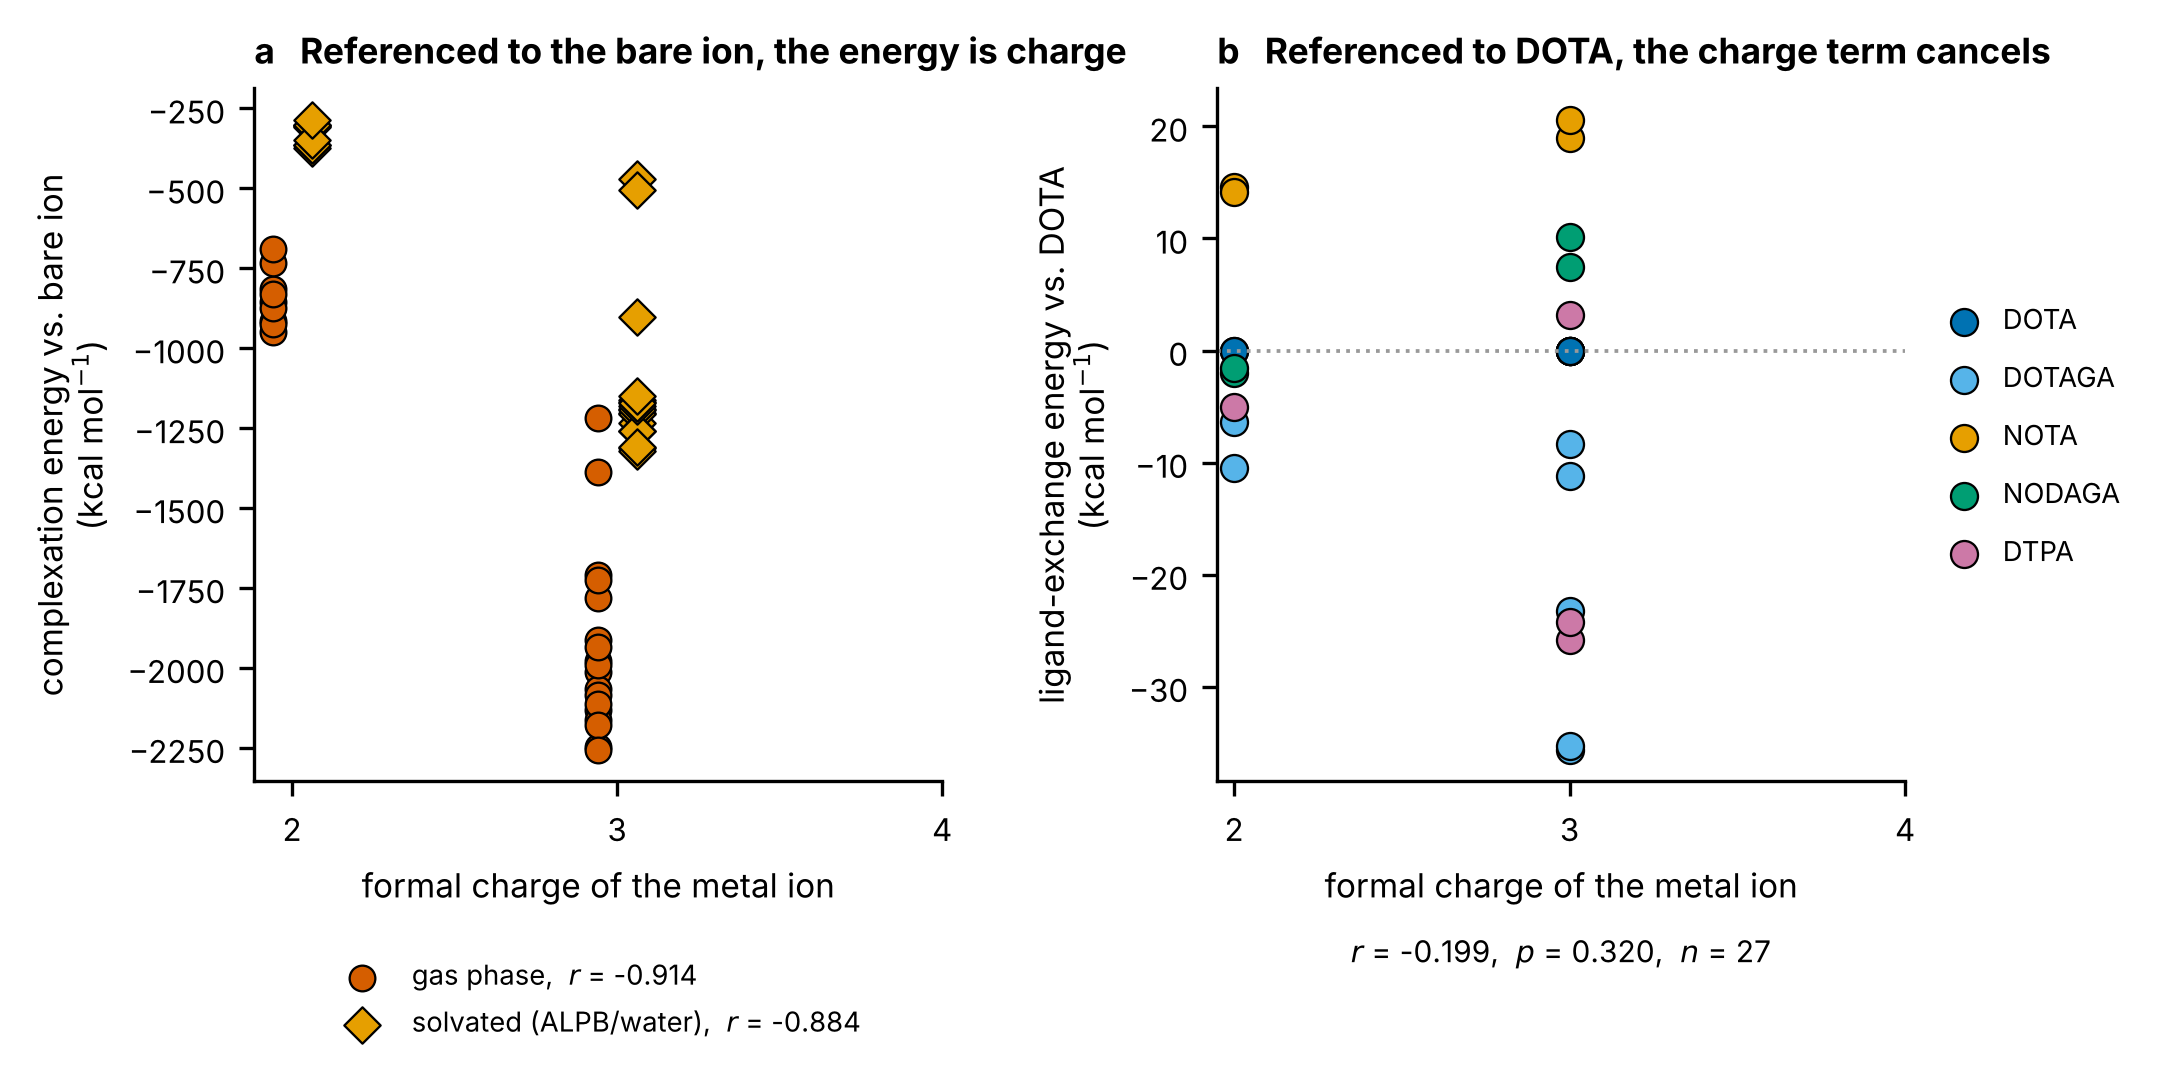
\includegraphics[width=\textwidth]{FigS1.png}
\caption{\textbf{The charge artefact and its removal.} (\textbf{a})~Complexation energies referenced
to the bare metal ion, for all 27 metal-bearing complexes, against the formal charge of the metal.
The energies track the oxidation state in both the gas phase and under ALPB solvation.
(\textbf{b})~The same complexes under the ligand-exchange energy referenced to DOTA; the charge
dependence is gone and the remaining spread is chelator chemistry.}
\label{fig:S1}
\end{figure}

%%====================================================================
\section{Improving the physics widens the generalisation gap}
\label{sec:ladder}
%%====================================================================

Two independent improvements were made to the quantum-chemical arm: replacing the complexation
energy with the exchange energy, and replacing the gas-phase treatment with ALPB implicit solvation
in water. Because they are separable we evaluated all four combinations on the same 82 observations
(Fig.~\ref{fig:S2}, and Table~2 of the article).

Every step that makes the chemistry more defensible raises the in-sample fit and lowers the
held-out performance, on both axes independently and in every ordering. We read this as the
signature of a descriptor set that is resolving the dataset rather than the effect: better physics
gives the model more to fit locally and nothing more to carry across target families. It is the
reason we do not present the in-sample numbers as partial success.

\begin{figure}[htbp]
\centering
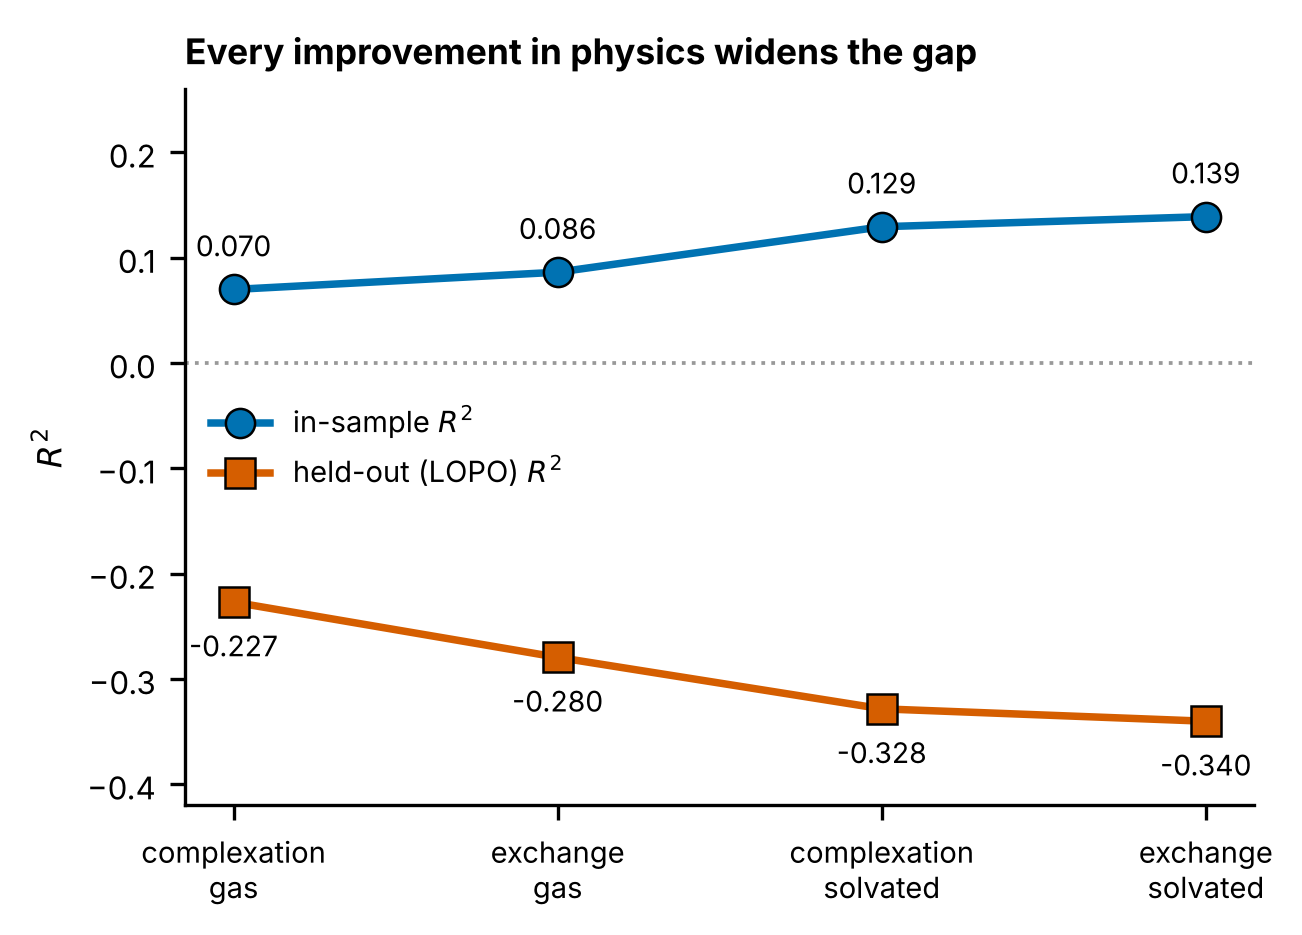
\includegraphics[width=0.62\textwidth]{FigS2.png}
\caption{\textbf{In-sample fit and held-out performance move in opposite directions.} Each point is
one of the four combinations of energy term and phase, fitted on the same 82 observations with the
same ridge pipeline. Leave-one-target-family-out validation throughout.}
\label{fig:S2}
\end{figure}

%%====================================================================
\section{What size of transferable effect the design could have caught}
%%====================================================================

A null result is only informative with a stated detection floor. We injected a synthetic effect that
is by construction a linear function of the descriptors---hence perfectly transferable, the most
favourable case a linear model could face---at a range of magnitudes, using 200 random descriptor
directions per magnitude, and recorded how often leave-one-target-family-out $R^2$ exceeded zero
(Fig.~\ref{fig:S3}).

The design detects a transferable twofold effect about three times in four, reaches 80\,\% only near
fourfold, and has essentially no power below roughly 1.4-fold. Because the injected effect was
linear in the descriptors, that floor is optimistic: a transferable effect with any non-linear
structure would need to be larger still. The effects actually present in the data have a median
magnitude of 1.50-fold within matched sets and reach 5.5-fold, so effects of the relevant size exist
here---they are simply not transferable.

\begin{figure}[htbp]
\centering
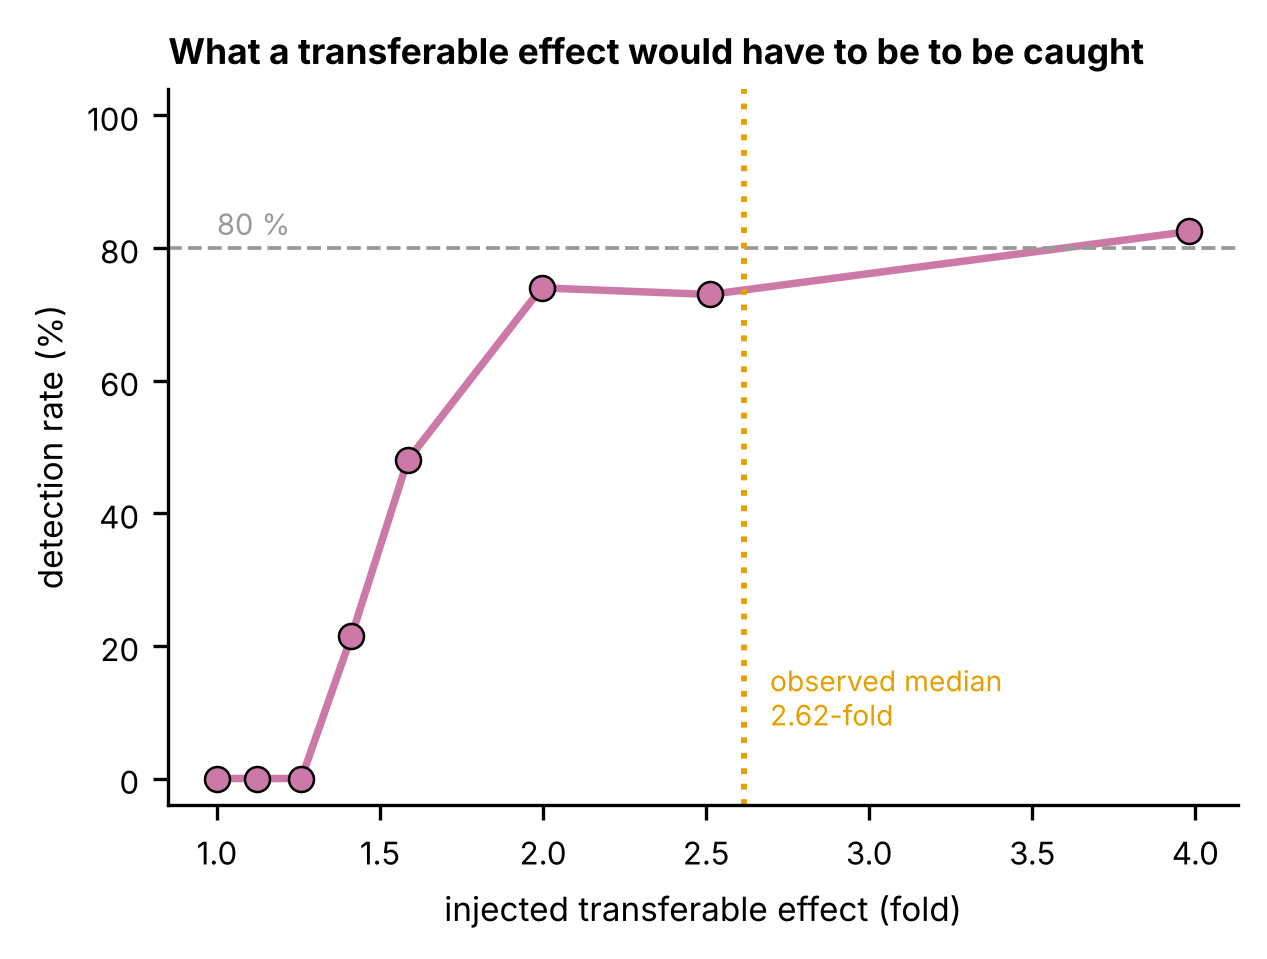
\includegraphics[width=0.62\textwidth]{FigS3.png}
\caption{\textbf{Injection power curve.} Detection rate against the magnitude of an injected
transferable effect, 200 random descriptor directions per magnitude. Dashed line, 80\,\% detection.
Dotted line, the median maximum/minimum affinity ratio actually observed within a matched set.}
\label{fig:S3}
\end{figure}

%%====================================================================
\section{Transfer under every grouping, both descriptor arms}
%%====================================================================

Leave-one-target-family-out is the validation the article reports, because target family is the
grouping a practitioner actually crosses when moving to a new construct. It is not the only
grouping that matters, and transfer fails under all of them (Fig.~\ref{fig:S4}).

The classical descriptors on the full 95 observations give $R^2 = -0.020$ for a held-out chelator,
$-0.088$ for a held-out vector, $-0.086$ for a held-out paper, $-0.177$ for a held-out target family
and $-0.187$ for a held-out metal. Adding the quantum-chemical descriptors on the 82 rows that carry
them makes every level worse. The held-out-chelator result for the combined arm ($-0.935$) is the
most extreme because only five chelators carry quantum-chemical coverage, so each fold removes a
large fraction of the descriptor range; we report it for completeness rather than as a separate
finding.

\begin{figure}[htbp]
\centering
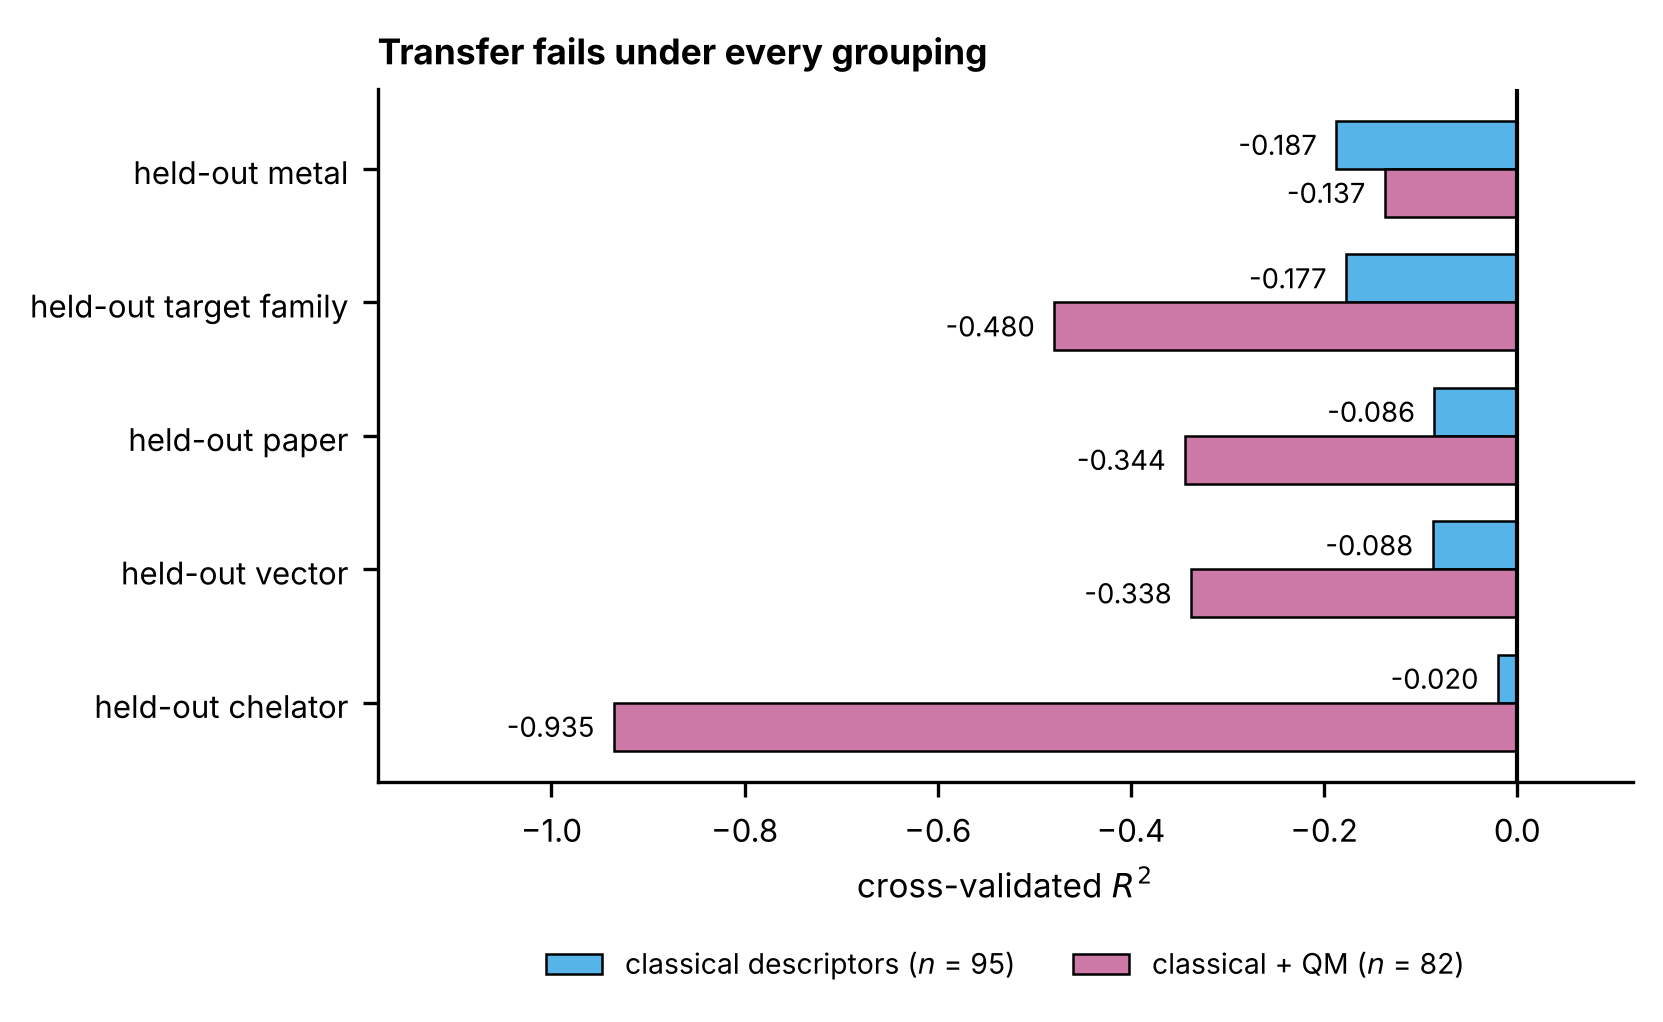
\includegraphics[width=0.72\textwidth]{FigS4.png}
\caption{\textbf{No grouping of the data leaves a positive result.} Cross-validated $R^2$ under five
held-out grouping schemes, for the classical descriptors on the full dataset and for the combined
classical and quantum-chemical descriptors on the subset carrying quantum-chemical coverage.}
\label{fig:S4}
\end{figure}

\clearpage
%%====================================================================
\section{Complete matched affinity dataset}
%%====================================================================

Table~\ref{tab:S1} lists all 106 transcribed affinity values with their source DOIs. Ninety-five of
these fall in 32 matched sets---one paper, one vector, one metal, one endpoint, with the chelator
varying---and are the analysis population; the remainder are singletons retained for provenance.
Values that a source reproduced from earlier work were identified by their footnotes and excluded as
duplicates: three pentixafor studies share one underlying dataset.

\small
\begin{longtable}{@{}p{1.8cm}p{3.0cm}p{1.7cm}p{0.9cm}p{1.2cm}r@{\hskip 10pt}r@{\hskip 12pt}p{3.3cm}@{}}
\caption{Complete matched affinity dataset. Every value was transcribed by hand from the open-access full text of the cited study; no value was parsed automatically, interpolated or estimated. Metal `---' denotes the metal-free conjugate.}\label{tab:S1}\\
\toprule
Family & Vector & Chelator & Metal & Endpoint & Value (nM) & SD & Source DOI \\
\midrule \endfirsthead
\multicolumn{8}{@{}l}{\small\itshape Table S1 continued}\\ \toprule
Family & Vector & Chelator & Metal & Endpoint & Value (nM) & SD & Source DOI \\
\midrule \endhead
\bottomrule \endlastfoot
CXCR4 & pentixafor\_scaffold & DFO\_Bn & \ce{Zr} & IC50 & 148 & 27 & \tiny{10.1186/s13550-016-0193-8} \\
CXCR4 & pentixafor\_scaffold & DFO\_Bn & --- & IC50 & 105 & 35 & \tiny{10.1186/s13550-016-0193-8} \\
CXCR4 & pentixafor\_scaffold & DOTA & \ce{Bi} & IC50 & 22.1 & 7 & \tiny{10.1186/s13550-016-0193-8} \\
CXCR4 & pentixafor\_scaffold & DOTA & \ce{Cu} & IC50 & 131 & 11 & \tiny{10.1186/s13550-016-0193-8} \\
CXCR4 & pentixafor\_scaffold & DOTA & \ce{Ga} & IC50 & 24.8 & 2.5 & \tiny{10.1186/s13550-016-0193-8} \\
CXCR4 & pentixafor\_scaffold & DOTA & \ce{Lu} & IC50 & 40.9 & 12 & \tiny{10.1186/s13550-016-0193-8} \\
CXCR4 & pentixafor\_scaffold & DOTA & \ce{Y} & IC50 & 40.8 & 27 & \tiny{10.1186/s13550-016-0193-8} \\
CXCR4 & pentixafor\_scaffold & DOTA & --- & IC50 & 102 & 17 & \tiny{10.1186/s13550-016-0193-8} \\
CXCR4 & pentixafor\_scaffold & DOTAGA & \ce{Bi} & IC50 & 29.4 & 7.6 & \tiny{10.1186/s13550-016-0193-8} \\
CXCR4 & pentixafor\_scaffold & DOTAGA & \ce{Cu} & IC50 & 1165 & 220 & \tiny{10.1186/s13550-016-0193-8} \\
CXCR4 & pentixafor\_scaffold & DOTAGA & \ce{Ga} & IC50 & 380 & 102 & \tiny{10.1186/s13550-016-0193-8} \\
CXCR4 & pentixafor\_scaffold & DOTAGA & \ce{Lu} & IC50 & 188 & 2.8 & \tiny{10.1186/s13550-016-0193-8} \\
CXCR4 & pentixafor\_scaffold & DOTAGA & \ce{Y} & IC50 & 126 & 89 & \tiny{10.1186/s13550-016-0193-8} \\
CXCR4 & pentixafor\_scaffold & DOTAGA & --- & IC50 & 654 & 263 & \tiny{10.1186/s13550-016-0193-8} \\
CXCR4 & pentixafor\_scaffold & DTPA & \ce{Cu} & IC50 & 175 & 66 & \tiny{10.1186/s13550-016-0193-8} \\
CXCR4 & pentixafor\_scaffold & DTPA & \ce{In} & IC50 & 90 & 42 & \tiny{10.1186/s13550-016-0193-8} \\
CXCR4 & pentixafor\_scaffold & DTPA & \ce{Lu} & IC50 & 111 & 77 & \tiny{10.1186/s13550-016-0193-8} \\
CXCR4 & pentixafor\_scaffold & DTPA & \ce{Y} & IC50 & 156 & 6.7 & \tiny{10.1186/s13550-016-0193-8} \\
CXCR4 & pentixafor\_scaffold & DTPA & --- & IC50 & 53 & 7.9 & \tiny{10.1186/s13550-016-0193-8} \\
CXCR4 & pentixafor\_scaffold & DTPA\_Bn & \ce{In} & IC50 & 74.1 & 2.4 & \tiny{10.1186/s13550-016-0193-8} \\
CXCR4 & pentixafor\_scaffold & DTPA\_Bn & --- & IC50 & 200 & 73 & \tiny{10.1186/s13550-016-0193-8} \\
CXCR4 & pentixafor\_scaffold & NODAGA & \ce{Cu} & IC50 & 343 & 10 & \tiny{10.1186/s13550-016-0193-8} \\
CXCR4 & pentixafor\_scaffold & NODAGA & \ce{Ga} & IC50 & 342 & 72 & \tiny{10.1186/s13550-016-0193-8} \\
CXCR4 & pentixafor\_scaffold & NODAGA & --- & IC50 & 275 & 106 & \tiny{10.1186/s13550-016-0193-8} \\
CXCR4 & pentixafor\_scaffold & NODA\_Bn & [\ce{AlF}]$^{2+}$ & IC50 & 329 & 49 & \tiny{10.1186/s13550-016-0193-8} \\
CXCR4 & pentixafor\_scaffold & NODA\_Bn & --- & IC50 & 115 & 24 & \tiny{10.1186/s13550-016-0193-8} \\
CXCR4 & pentixafor\_scaffold & NOTA & [\ce{AlF}]$^{2+}$ & IC50 & 220 & 57 & \tiny{10.1186/s13550-016-0193-8} \\
CXCR4 & pentixafor\_scaffold & NOTA & \ce{Cu} & IC50 & 46.1 & 26 & \tiny{10.1186/s13550-016-0193-8} \\
CXCR4 & pentixafor\_scaffold & NOTA & \ce{Ga} & IC50 & 17.8 & 7.7 & \tiny{10.1186/s13550-016-0193-8} \\
CXCR4 & pentixafor\_scaffold & NOTA & --- & IC50 & 253 & 49 & \tiny{10.1186/s13550-016-0193-8} \\
CXCR4 & pentixather\_scaffold & NODAGA & \ce{Cu} & IC50 & 47.5 & 1.8 & \tiny{10.1186/s41181-016-0020-6} \\
CXCR4 & pentixather\_scaffold & NODAGA & --- & IC50 & 64.9 & 6.5 & \tiny{10.1186/s41181-016-0020-6} \\
CXCR4 & pentixather\_scaffold & NOTA & \ce{Cu} & IC50 & 14.9 & 2.1 & \tiny{10.1186/s41181-016-0020-6} \\
CXCR4 & pentixather\_scaffold & NOTA & --- & IC50 & 27.5 & 2.1 & \tiny{10.1186/s41181-016-0020-6} \\
GRPR & PEG2-RM26 & DOTA & \ce{Co} & IC50 & 2 & 0.2 & \tiny{10.1038/s41598-019-52914-y} \\
GRPR & PEG2-RM26 & DOTA & \ce{Co} & KD & 0.033 & 0.012 & \tiny{10.1038/s41598-019-52914-y} \\
GRPR & PEG2-RM26 & DOTAGA & \ce{Co} & IC50 & 4.4 & 0.4 & \tiny{10.1038/s41598-019-52914-y} \\
GRPR & PEG2-RM26 & DOTAGA & \ce{Co} & KD & 0.167 & 0.022 & \tiny{10.1038/s41598-019-52914-y} \\
GRPR & PEG2-RM26 & NODAGA & \ce{Co} & IC50 & 4.7 & 0.7 & \tiny{10.1038/s41598-019-52914-y} \\
GRPR & PEG2-RM26 & NODAGA & \ce{Co} & KD & 0.066 & 0.025 & \tiny{10.1038/s41598-019-52914-y} \\
GRPR & PEG2-RM26 & NOTA & \ce{Co} & IC50 & 2.8 & 0.2 & \tiny{10.1038/s41598-019-52914-y} \\
GRPR & PEG2-RM26 & NOTA & \ce{Co} & KD & 0.056 & 0.003 & \tiny{10.1038/s41598-019-52914-y} \\
GRPR & RM2 & DOTA & \ce{Cu} & IC50 & 3.2 & 0.6 & \tiny{10.1186/s13550-025-01241-7} \\
GRPR & RM2 & DOTA & \ce{Ga} & IC50 & 2.1 & 0.3 & \tiny{10.1186/s13550-025-01241-7} \\
GRPR & RM2 & DOTA & \ce{Lu} & IC50 & 3.5 & 0.2 & \tiny{10.1186/s13550-025-01241-7} \\
GRPR & RM2 & NODAGA & \ce{Cu} & IC50 & 3.1 & 0.4 & \tiny{10.1186/s13550-025-01241-7} \\
GRPR & RM2 & NODAGA & \ce{Ga} & IC50 & 1.4 & 0.2 & \tiny{10.1186/s13550-025-01241-7} \\
GRPR & RM2 & NOTA & \ce{Cu} & IC50 & 1.7 & 0.3 & \tiny{10.1186/s13550-025-01241-7} \\
GRPR & RM2 & NOTA & \ce{Ga} & IC50 & 1.2 & 0.1 & \tiny{10.1186/s13550-025-01241-7} \\
GRPR & RM2\_Bta8 & DOTA & \ce{Cu} & IC50 & 4.2 & 0.6 & \tiny{10.1186/s13550-025-01241-7} \\
GRPR & RM2\_Bta8 & DOTA & \ce{Ga} & IC50 & 2.3 & 0.1 & \tiny{10.1186/s13550-025-01241-7} \\
GRPR & RM2\_Bta8 & DOTA & \ce{Lu} & IC50 & 4.6 & 0.2 & \tiny{10.1186/s13550-025-01241-7} \\
GRPR & RM2\_Bta8 & NODAGA & \ce{Cu} & IC50 & 8.9 & 0.3 & \tiny{10.1186/s13550-025-01241-7} \\
GRPR & RM2\_Bta8 & NODAGA & \ce{Ga} & IC50 & 2.9 & 0.6 & \tiny{10.1186/s13550-025-01241-7} \\
GRPR & RM2\_Bta8 & NOTA & \ce{Cu} & IC50 & 2.8 & 0.2 & \tiny{10.1186/s13550-025-01241-7} \\
GRPR & RM2\_Bta8 & NOTA & \ce{Ga} & IC50 & 1.8 & 0 & \tiny{10.1186/s13550-025-01241-7} \\
GRPR & RM2\_Hse7 & DOTA & \ce{Cu} & IC50 & 33 & 2.7 & \tiny{10.1186/s13550-025-01241-7} \\
GRPR & RM2\_Hse7 & DOTA & \ce{Ga} & IC50 & 7.7 & 0.7 & \tiny{10.1186/s13550-025-01241-7} \\
GRPR & RM2\_Hse7 & DOTA & \ce{Lu} & IC50 & 19.7 & 1.6 & \tiny{10.1186/s13550-025-01241-7} \\
GRPR & RM2\_Hse7 & NODAGA & \ce{Cu} & IC50 & 11.8 & 2.1 & \tiny{10.1186/s13550-025-01241-7} \\
GRPR & RM2\_Hse7 & NODAGA & \ce{Ga} & IC50 & 7.2 & 0.7 & \tiny{10.1186/s13550-025-01241-7} \\
GRPR & RM2\_Hse7 & NOTA & \ce{Cu} & IC50 & 14.2 & 2.7 & \tiny{10.1186/s13550-025-01241-7} \\
GRPR & RM2\_Hse7 & NOTA & \ce{Ga} & IC50 & 8.4 & 1 & \tiny{10.1186/s13550-025-01241-7} \\
GRPR & RM2\_aMeTrp8 & DOTA & \ce{Cu} & IC50 & 4 & 0.5 & \tiny{10.1186/s13550-025-01241-7} \\
GRPR & RM2\_aMeTrp8 & DOTA & \ce{Ga} & IC50 & 1.5 & 0.2 & \tiny{10.1186/s13550-025-01241-7} \\
GRPR & RM2\_aMeTrp8 & DOTA & \ce{Lu} & IC50 & 3 & 0 & \tiny{10.1186/s13550-025-01241-7} \\
GRPR & RM2\_aMeTrp8 & NODAGA & \ce{Cu} & IC50 & 12.6 & 0.4 & \tiny{10.1186/s13550-025-01241-7} \\
GRPR & RM2\_aMeTrp8 & NODAGA & \ce{Ga} & IC50 & 4.9 & 0.7 & \tiny{10.1186/s13550-025-01241-7} \\
GRPR & RM2\_aMeTrp8 & NOTA & \ce{Cu} & IC50 & 5.1 & 0.3 & \tiny{10.1186/s13550-025-01241-7} \\
GRPR & RM2\_aMeTrp8 & NOTA & \ce{Ga} & IC50 & 5 & 0.7 & \tiny{10.1186/s13550-025-01241-7} \\
PSMA & Ahx-KuE & HBED\_CC & \ce{Ga} & IC50 & 6.1 & 0.8 & \tiny{10.1186/s13550-014-0063-1} \\
PSMA & Ahx-KuE & HBED\_CC & --- & IC50 & 5.7 & 0.5 & \tiny{10.1186/s13550-014-0063-1} \\
PSMA & FFK\_SubKuE & DOTA & \ce{Ga} & IC50 & 29.5 & 6.6 & \tiny{10.1186/s13550-014-0063-1} \\
PSMA & FFK\_SubKuE & DOTA & \ce{Lu} & IC50 & 54.7 & 6.1 & \tiny{10.1186/s13550-014-0063-1} \\
PSMA & FFK\_SubKuE & DOTA & --- & IC50 & 13.1 & 2.3 & \tiny{10.1186/s13550-014-0063-1} \\
PSMA & FFK\_SubKuE & DOTAGA & \ce{Ga} & IC50 & 12.1 & 3.9 & \tiny{10.1186/s13550-014-0063-1} \\
PSMA & FFK\_SubKuE & DOTAGA & \ce{Lu} & IC50 & 15.1 & 1.5 & \tiny{10.1186/s13550-014-0063-1} \\
PSMA & FFK\_SubKuE & DOTAGA & --- & IC50 & 10.2 & 1.5 & \tiny{10.1186/s13550-014-0063-1} \\
PSMA & PSMA-617 & AAZTA5 & \ce{Ga} & Ki & 8.7 & 0.9 & \tiny{10.1186/s41181-020-00107-8} \\
PSMA & PSMA-617 & AAZTA5 & \ce{Lu} & Ki & 26.6 & 11.1 & \tiny{10.1186/s41181-020-00107-8} \\
PSMA & PSMA-617 & AAZTA5 & \ce{Sc} & Ki & 30.6 & 11.5 & \tiny{10.1186/s41181-020-00107-8} \\
PSMA & PSMA-617 & DOTA & \ce{Ga} & Ki & 6.4 & 1 & \tiny{10.1186/s41181-020-00107-8} \\
PSMA & PSMA-617 & DOTA & \ce{Lu} & Ki & 6.9 & 1.3 & \tiny{10.1186/s41181-020-00107-8} \\
PSMA & PSMA-617 & DOTA & \ce{Sc} & Ki & 4.7 & 0.8 & \tiny{10.1186/s41181-020-00107-8} \\
PSMA & PSMA-I\&T & DOTAGA & \ce{Cu} & IC50 & 11.2 & 2.3 & \tiny{10.2967/jnumed.123.267126} \\
PSMA & PSMA-I\&T & NODAGA & \ce{Cu} & IC50 & 9.3 & 1.8 & \tiny{10.2967/jnumed.123.267126} \\
PSMA & ffk\_SubKuE & DOTAGA & \ce{Ga} & IC50 & 15.9 & 0.5 & \tiny{10.1186/s13550-014-0063-1} \\
PSMA & ffk\_SubKuE & DOTAGA & \ce{Lu} & IC50 & 13.1 & 2.2 & \tiny{10.1186/s13550-014-0063-1} \\
PSMA & ffk\_SubKuE & DOTAGA & --- & IC50 & 13.9 & 0.4 & \tiny{10.1186/s13550-014-0063-1} \\
SSTR & TOC & DOTA & \ce{Cu} & IC50 & 0.23 &  & \tiny{10.3389/fnume.2024.1481343} \\
SSTR & TOC & DOTA & \ce{Cu} & KD & 0.105 & 0.011 & \tiny{10.3389/fnume.2024.1481343} \\
SSTR & TOC & DOTA & \ce{Ga} & IC50 & 0.18 &  & \tiny{10.3389/fnume.2024.1481343} \\
SSTR & TOC & NODAGA & \ce{Cu} & IC50 & 0.34 &  & \tiny{10.3389/fnume.2024.1481343} \\
SSTR & TOC & NODAGA & \ce{Cu} & KD & 0.078 & 0.007 & \tiny{10.3389/fnume.2024.1481343} \\
affibody & Z08698 & DOTA & \ce{In} & KD & 0.08 &  & \tiny{10.1038/s41598-018-36827-w} \\
affibody & Z08698 & DOTA & --- & KD & 0.012 &  & \tiny{10.1038/s41598-018-36827-w} \\
affibody & Z08698 & DOTAGA & \ce{In} & KD & 0.008 &  & \tiny{10.1038/s41598-018-36827-w} \\
affibody & Z08698 & DOTAGA & --- & KD & 0.015 &  & \tiny{10.1038/s41598-018-36827-w} \\
affibody & Z08698 & NODAGA & \ce{In} & KD & 0.021 &  & \tiny{10.1038/s41598-018-36827-w} \\
affibody & Z08698 & NODAGA & --- & KD & 0.011 &  & \tiny{10.1038/s41598-018-36827-w} \\
affibody & Z08698 & NOTA & \ce{In} & KD & 0.16 &  & \tiny{10.1038/s41598-018-36827-w} \\
affibody & Z08698 & NOTA & --- & KD & 0.04 &  & \tiny{10.1038/s41598-018-36827-w} \\
affibody & Z\_HER3\_affibody & DOTA & \ce{Co} & KD & 0.2 & 0.1 & \tiny{10.3390/ijms21061972} \\
affibody & Z\_HER3\_affibody & DOTAGA & \ce{Co} & KD & 0.2 & 0.1 & \tiny{10.3390/ijms21061972} \\
affibody & Z\_HER3\_affibody & NODAGA & \ce{Co} & KD & 0.09 & 0.07 & \tiny{10.3390/ijms21061972} \\
affibody & Z\_HER3\_affibody & NOTA & \ce{Co} & KD & 0.1 & 0.1 & \tiny{10.3390/ijms21061972} \\
\bottomrule
\end{longtable}
\normalsize

\clearpage
%%====================================================================
\section{Optimised complexes and coordination verification}
%%====================================================================

Table~\ref{tab:S2} lists all 32 metal--chelate combinations, of which 27 carry a metal. Coordination
mode was verified against the mode known for each chelator rather than assumed: Ga--DOTA as
N$_4$O$_3$ with Ga--O 1.84--1.94\,\AA{} and Ga--N 2.26--2.54\,\AA, Ga--NODAGA as N$_3$O$_3$,
Lu--DOTA as N$_4$O$_4$, and so on. All 27 passed. Five starting structures were used per complex
(four fresh conformer seeds plus a re-relaxation of a gas-phase optimum) and the lowest-energy
structure \emph{with a chemically valid coordination mode} was kept---not the lowest-energy
structure outright. Five complexes (Lu--DOTA, Lu--DOTAGA, Y--DOTAGA, Cu--DTPA, Lu--DTPA) initially
failed this check and were re-run with a twelve-seed sweep rather than by relaxing the criterion.

Solvation changed the structures materially: four of 27 coordination numbers shifted, the mean M--N
distance contracted by 0.10\,\AA, and the mean dipole moment rose from 16.0 to 25.9\,D. Cartesian
coordinates for every complex, gas-phase and solvated, are in the deposited archive.

\small
\begin{longtable}{@{}p{1.6cm}p{1.2cm}r@{\hskip 10pt}r@{\hskip 10pt}l@{\hskip 10pt}c@{\hskip 10pt}r@{\hskip 10pt}r@{\hskip 10pt}r@{}}
\caption{Optimised metal--chelate complexes (GFN2-xTB with ALPB implicit solvation in water). `Coord.\ verified' records whether the optimised coordination mode matched the mode known for that chelator; all 27 metal-bearing complexes passed. The ligand-exchange energy is referenced to DOTA at the same metal, so it is zero by definition for DOTA and undefined for the metal-free ligands.}\label{tab:S2}\\
\toprule
Chelator & Metal & Charge & Atoms & CN & Coord.\ verified & $\Delta\Delta E$ (kcal\,mol$^{-1}$) & $\mu$ (D) & $q_\mathrm{M}$ \\
\midrule \endfirsthead
\multicolumn{9}{@{}l}{\small\itshape Table S2 continued}\\ \toprule
Chelator & Metal & Charge & Atoms & CN & Coord.\ verified & $\Delta\Delta E$ (kcal\,mol$^{-1}$) & $\mu$ (D) & $q_\mathrm{M}$ \\
\midrule \endhead
\bottomrule \endlastfoot
DOTA & \ce{Bi} & +0 & 58 & 7 (N$_{4}$O$_{3}$) & \checkmark & 0 (ref.) & 17.3 & +1.027 \\
DOTA & \ce{Co} & -1 & 58 & 6 (N$_{4}$O$_{2}$) & \checkmark & 0 (ref.) & 14.1 & +0.072 \\
DOTA & \ce{Cu} & -1 & 58 & 5 (N$_{3}$O$_{2}$) & \checkmark & 0 (ref.) & 10.8 & +0.381 \\
DOTA & \ce{Ga} & +0 & 58 & 7 (N$_{4}$O$_{3}$) & \checkmark & 0 (ref.) & 25.2 & +0.066 \\
DOTA & \ce{In} & +0 & 58 & 7 (N$_{4}$O$_{3}$) & \checkmark & 0 (ref.) & 19.9 & +0.283 \\
DOTA & \ce{Lu} & +0 & 58 & 8 (N$_{4}$O$_{4}$) & \checkmark & 0 (ref.) & 23.7 & +0.761 \\
DOTA & \ce{Sc} & +0 & 58 & 7 (N$_{4}$O$_{3}$) & \checkmark & 0 (ref.) & 22.3 & +0.805 \\
DOTA & \ce{Y} & +0 & 58 & 7 (N$_{4}$O$_{3}$) & \checkmark & 0 (ref.) & 21.3 & +0.671 \\
DOTA & --- & -3 & 57 & --- & --- & --- & 21.4 & --- \\
DOTAGA & \ce{Bi} & -1 & 66 & 8 (N$_{4}$O$_{4}$) & \checkmark & -35.7 & 32.2 & +1.047 \\
DOTAGA & \ce{Co} & -2 & 66 & 6 (N$_{3}$O$_{3}$) & \checkmark & -10.5 & 27.7 & +0.096 \\
DOTAGA & \ce{Cu} & -2 & 66 & 6 (N$_{3}$O$_{3}$) & \checkmark & -6.3 & 29.0 & +0.416 \\
DOTAGA & \ce{Ga} & -1 & 66 & 8 (N$_{4}$O$_{4}$) & \checkmark & -11.2 & 38.3 & +0.051 \\
DOTAGA & \ce{In} & -1 & 66 & 8 (N$_{4}$O$_{4}$) & \checkmark & -35.3 & 40.2 & +0.276 \\
DOTAGA & \ce{Lu} & -1 & 66 & 8 (N$_{4}$O$_{4}$) & \checkmark & -23.3 & 35.7 & +0.782 \\
DOTAGA & \ce{Y} & -1 & 66 & 8 (N$_{4}$O$_{4}$) & \checkmark & -8.3 & 26.1 & +0.659 \\
DOTAGA & --- & -4 & 65 & --- & --- & --- & 21.1 & --- \\
DTPA & \ce{Cu} & -2 & 51 & 6 (N$_{2}$O$_{4}$) & \checkmark & -5.0 & 36.3 & +0.497 \\
DTPA & \ce{In} & -1 & 51 & 8 (N$_{3}$O$_{5}$) & \checkmark & -25.8 & 41.8 & +0.264 \\
DTPA & \ce{Lu} & -1 & 51 & 8 (N$_{3}$O$_{5}$) & \checkmark & -24.3 & 33.1 & +0.796 \\
DTPA & \ce{Y} & -1 & 51 & 7 (N$_{3}$O$_{4}$) & \checkmark & +3.2 & 23.4 & +0.669 \\
DTPA & --- & -4 & 50 & --- & --- & --- & 29.1 & --- \\
NODAGA & \ce{Co} & -1 & 53 & 6 (N$_{3}$O$_{3}$) & \checkmark & -2.0 & 24.1 & +0.089 \\
NODAGA & \ce{Cu} & -1 & 53 & 6 (N$_{3}$O$_{3}$) & \checkmark & -1.6 & 31.2 & +0.442 \\
NODAGA & \ce{Ga} & +0 & 53 & 6 (N$_{3}$O$_{3}$) & \checkmark & +10.1 & 21.8 & +0.126 \\
NODAGA & \ce{In} & +0 & 53 & 6 (N$_{3}$O$_{3}$) & \checkmark & +7.5 & 18.4 & +0.332 \\
NODAGA & --- & -3 & 52 & --- & --- & --- & 36.3 & --- \\
NOTA & \ce{Co} & +0 & 45 & 5 (N$_{3}$O$_{2}$) & \checkmark & +14.6 & 21.3 & +0.104 \\
NOTA & \ce{Cu} & +0 & 45 & 5 (N$_{3}$O$_{2}$) & \checkmark & +14.2 & 26.0 & +0.445 \\
NOTA & \ce{Ga} & +1 & 45 & 6 (N$_{3}$O$_{3}$) & \checkmark & +19.0 & 23.6 & +0.131 \\
NOTA & \ce{In} & +1 & 45 & 6 (N$_{3}$O$_{3}$) & \checkmark & +20.6 & 15.5 & +0.330 \\
NOTA & --- & -2 & 44 & --- & --- & --- & 17.7 & --- \\
\bottomrule
\end{longtable}
\normalsize

\clearpage
%%====================================================================
\section{Lipophilicity as a confounder}
%%====================================================================

A chelator swap changes lipophilicity as well as sterics and charge, so a referee is right to ask
whether the affinity shifts are a lipophilicity effect in disguise. Every log$D_{7.4}$ or log$P$
value reported alongside the affinity data in the same tables was transcribed (Table~\ref{tab:S3};
38 values from four of the ten studies). Across the 29 within-set pairs for which both quantities
are available, the difference in lipophilicity explains 7.4\,\% of the difference in affinity and
the association is not significant ($r = +0.272$, $p = 0.153$, bootstrap 95\,\% CI
$[-0.146, +0.580]$). The absolute values are uncorrelated ($r = -0.040$, $p = 0.838$).

This does not establish that lipophilicity is irrelevant to conjugate design; it establishes that it
does not account for the effect audited here, on the subset of the data where it can be tested.

\small
\begin{longtable}{@{}p{3.0cm}p{1.7cm}p{1.0cm}r@{\hskip 14pt}p{3.4cm}p{3.2cm}@{}}
\caption{Reported lipophilicity values transcribed alongside the affinity data, used to test lipophilicity as a confounder.}\label{tab:S3}\\
\toprule Vector & Chelator & Metal & log$D$ / log$P$ & Note & Source DOI \\
\midrule \endfirsthead
\multicolumn{6}{@{}l}{\small\itshape Table S3 continued}\\ \toprule
Vector & Chelator & Metal & log$D$ / log$P$ & Note & Source DOI \\
\midrule \endhead
\bottomrule \endlastfoot
Ahx-KuE & HBED\_CC & \ce{Ga} & -4.1 & \tiny{} & \tiny{10.1186/s13550-014-0063-1} \\
FFK\_SubKuE & DOTA & \ce{Ga} & -3.1 & \tiny{} & \tiny{10.1186/s13550-014-0063-1} \\
FFK\_SubKuE & DOTA & \ce{Lu} & -2.7 & \tiny{} & \tiny{10.1186/s13550-014-0063-1} \\
FFK\_SubKuE & DOTAGA & \ce{Ga} & -3.6 & \tiny{reported as the sum over FFK/ffk isomers} & \tiny{10.1186/s13550-014-0063-1} \\
FFK\_SubKuE & DOTAGA & \ce{Lu} & -3.9 & \tiny{reported as the sum over FFK/ffk isomers} & \tiny{10.1186/s13550-014-0063-1} \\
RM2 & DOTA & \ce{Ga} & -2.78 & \tiny{} & \tiny{10.1186/s13550-025-01241-7} \\
RM2 & DOTA & \ce{Cu} & -2.37 & \tiny{} & \tiny{10.1186/s13550-025-01241-7} \\
RM2 & DOTA & \ce{Lu} & -2.51 & \tiny{} & \tiny{10.1186/s13550-025-01241-7} \\
RM2 & NODAGA & \ce{Ga} & -1.68 & \tiny{} & \tiny{10.1186/s13550-025-01241-7} \\
RM2 & NODAGA & \ce{Cu} & -2.14 & \tiny{} & \tiny{10.1186/s13550-025-01241-7} \\
RM2 & NOTA & \ce{Ga} & -1.93 & \tiny{} & \tiny{10.1186/s13550-025-01241-7} \\
RM2 & NOTA & \ce{Cu} & -2.26 & \tiny{} & \tiny{10.1186/s13550-025-01241-7} \\
RM2\_Bta8 & DOTA & \ce{Ga} & -2.32 & \tiny{} & \tiny{10.1186/s13550-025-01241-7} \\
RM2\_Bta8 & DOTA & \ce{Cu} & -1.73 & \tiny{} & \tiny{10.1186/s13550-025-01241-7} \\
RM2\_Bta8 & DOTA & \ce{Lu} & -1.81 & \tiny{} & \tiny{10.1186/s13550-025-01241-7} \\
RM2\_Bta8 & NODAGA & \ce{Ga} & -1.14 & \tiny{} & \tiny{10.1186/s13550-025-01241-7} \\
RM2\_Bta8 & NODAGA & \ce{Cu} & -1.62 & \tiny{} & \tiny{10.1186/s13550-025-01241-7} \\
RM2\_Bta8 & NOTA & \ce{Ga} & -1.28 & \tiny{} & \tiny{10.1186/s13550-025-01241-7} \\
RM2\_Bta8 & NOTA & \ce{Cu} & -1.59 & \tiny{} & \tiny{10.1186/s13550-025-01241-7} \\
RM2\_Hse7 & DOTA & \ce{Ga} & -2.9 & \tiny{} & \tiny{10.1186/s13550-025-01241-7} \\
RM2\_Hse7 & DOTA & \ce{Cu} & -2.04 & \tiny{} & \tiny{10.1186/s13550-025-01241-7} \\
RM2\_Hse7 & DOTA & \ce{Lu} & -2.25 & \tiny{} & \tiny{10.1186/s13550-025-01241-7} \\
RM2\_Hse7 & NODAGA & \ce{Ga} & -1.51 & \tiny{} & \tiny{10.1186/s13550-025-01241-7} \\
RM2\_Hse7 & NODAGA & \ce{Cu} & -2 & \tiny{} & \tiny{10.1186/s13550-025-01241-7} \\
RM2\_Hse7 & NOTA & \ce{Ga} & -1.56 & \tiny{} & \tiny{10.1186/s13550-025-01241-7} \\
RM2\_Hse7 & NOTA & \ce{Cu} & -1.95 & \tiny{} & \tiny{10.1186/s13550-025-01241-7} \\
RM2\_aMeTrp8 & DOTA & \ce{Ga} & -2.26 & \tiny{} & \tiny{10.1186/s13550-025-01241-7} \\
RM2\_aMeTrp8 & DOTA & \ce{Cu} & -2.17 & \tiny{} & \tiny{10.1186/s13550-025-01241-7} \\
RM2\_aMeTrp8 & DOTA & \ce{Lu} & -2.28 & \tiny{} & \tiny{10.1186/s13550-025-01241-7} \\
RM2\_aMeTrp8 & NODAGA & \ce{Ga} & -1.42 & \tiny{} & \tiny{10.1186/s13550-025-01241-7} \\
RM2\_aMeTrp8 & NODAGA & \ce{Cu} & -1.94 & \tiny{} & \tiny{10.1186/s13550-025-01241-7} \\
RM2\_aMeTrp8 & NOTA & \ce{Ga} & -1.41 & \tiny{} & \tiny{10.1186/s13550-025-01241-7} \\
RM2\_aMeTrp8 & NOTA & \ce{Cu} & -1.79 & \tiny{} & \tiny{10.1186/s13550-025-01241-7} \\
PSMA-I\&T & DOTAGA & \ce{Cu} & -2.69 & \tiny{} & \tiny{10.2967/jnumed.123.267126} \\
PSMA-I\&T & NODAGA & \ce{Cu} & -2.95 & \tiny{} & \tiny{10.2967/jnumed.123.267126} \\
TOC & DOTA & \ce{Cu} & -2.81 & \tiny{} & \tiny{10.3389/fnume.2024.1481343} \\
TOC & DOTA & \ce{Ga} & -3.18 & \tiny{} & \tiny{10.3389/fnume.2024.1481343} \\
TOC & NODAGA & \ce{Cu} & -2.6 & \tiny{} & \tiny{10.3389/fnume.2024.1481343} \\
\bottomrule
\end{longtable}
\normalsize

\clearpage
%%====================================================================
\section{Software, reproducibility and deposited files}
%%====================================================================

Calculations used GFN2-xTB through \textsf{tblite} with the ASE interface, with ALPB implicit
solvation in water, at the correct total charge and spin multiplicity for each complex. Structures
were built from SMILES with RDKit; metals were threaded into the macrocyclic cavity using explicit
dative bonds to the ring nitrogens and carboxylate oxygens \emph{before} 3-D embedding, because
embedding first allows the ion to escape the cavity. Statistical analysis used scikit-learn,
SciPy, NumPy and pandas. Exact versions are pinned in \texttt{requirements.txt} in the archive.

Confidence intervals come from 10\,000 bootstrap resamples. The within-set label-permutation null
uses 2000 permutations. Random seeds are fixed in every script; the pairwise analyses and the
permutation test each state their seed in the file they write.

The archive contains the raw affinity table with per-row DOI provenance, the derived analysis table,
the classical and quantum-chemical descriptor tables, the ligand-exchange energies, the optimised
Cartesian geometries of all 32 complexes in both the gas phase and solvated, the screened candidate
pool, the lipophilicity table, and the complete analysis pipeline. Running the pipeline from the
deposited files reproduces every number and figure in the article and in this document.

%%====================================================================
\section*{References}
%%====================================================================

\begin{enumerate}\setlength{\itemsep}{2pt}
\item C.~Bannwarth, S.~Ehlert and S.~Grimme, \textit{J. Chem. Theory Comput.}, 2019, \textbf{15}, 1652--1671.
\item C.~Bannwarth, E.~Caldeweyher, S.~Ehlert, A.~Hansen, P.~Pracht, J.~Seibert, S.~Spicher and S.~Grimme, \textit{WIREs Comput. Mol. Sci.}, 2021, \textbf{11}, e1493.
\item S.~Ehlert, M.~St{\"a}hn, S.~Spicher and S.~Grimme, \textit{J. Chem. Theory Comput.}, 2021, \textbf{17}, 4250--4261.
\item P.~Pracht, S.~Grimme, C.~Bannwarth, F.~Bohle, S.~Ehlert, G.~Feldmann, J.~Gorges, M.~M{\"u}ller, T.~Neudecker, C.~Plett, S.~Spicher, P.~Steinbach, P.~A.~Wesołowski and F.~Zeller, \textit{J. Chem. Phys.}, 2024, \textbf{160}, 114110.
\item E.~W.~Price and C.~Orvig, \textit{Chem. Soc. Rev.}, 2014, \textbf{43}, 260--290.
\end{enumerate}

\end{document}
